\documentclass[a4paper,12pt]{article}
\usepackage[margin=3cm]{geometry}
\usepackage[slovene]{babel}
\usepackage[utf8]{inputenc}
\usepackage[T1]{fontenc}
\usepackage{lmodern}
\usepackage{url}
\usepackage{graphicx}
\usepackage{amsmath}
\usepackage{amssymb}
\usepackage{amsfonts}
\usepackage{hyperref}
\usepackage{amsthm}
\usepackage{pgfpages}
\usepackage{colortbl}
\usepackage{tikz}
\usepackage{array}
\usepackage{amsmath,amsthm, amsfonts,amssymb}
\usepackage{mathtools}
\usepackage{tikz}

\usepackage{natbib} % or use \usepackage{biblatex} if you prefer to use biblatex
%\bibliography{Naloga-Anej-Rozman.bib} % replace example.bib with the name of your .bib file


\usetikzlibrary{positioning}
\usetikzlibrary{automata}


\def\N{\mathbb{N}} % mnozica naravnih stevil
\def\Z{\mathbb{Z}} % mnozica celih stevil
\def\Q{\mathbb{Q}} % mnozica racionalnih stevil
\def\R{\mathbb{R}} % mnozica realnih stevil
\def\C{\mathbb{C}} % mnozica kompleksnih stevil

\newcommand{\geslo}[2]{\noindent\textbf{#1} \quad \hangindent=1cm #2\\[-1pc]}

\def\qed{$\hfill\Box$}   % konec dokaza
\def\qedm{\qquad\Box}   % konec dokaza v matematičnem načinu
\newtheorem{izrek}{Izrek}[section]
\newtheorem{trditev}[izrek]{Trditev}
\newtheorem{posledica}[izrek]{Posledica}
\newtheorem{lema}[izrek]{Lema}
\newtheorem{opomba}[izrek]{Opomba}
\newtheorem{definicija}[izrek]{Definicija}
\newtheorem{zgled}[izrek]{Zgled}



\begin{document}

\begin{titlepage}
UNIVERZA V LJUBLJANI

FAKULTETA ZA MATEMATIKO IN FIZIKO

\vspace{0.5cm}
Finančna matematika - 1. stopnja

\begin{center}
   \vspace{7cm}
   Anej Rozman

   \vspace{0.4cm}
   \textbf{\Large{O klasifikaciji stanj v markovskih verigah}}
   \vspace{0.3cm}

   Delo pri predmetu seminar

   \vspace{1cm}
   Mentor: doc.\@ dr.\@ Martin Raič
\end{center}
\vfill
Ljubljana, 2023     
\thispagestyle{empty}
\end{titlepage}
\newpage

\tableofcontents


\newpage

\section{Uvod}

Markovske verige so matematični model, ki se uporablja za opisovanje naključnih procesov, kjer je prihodnje stanje sistema odvisno le od trenutnega stanja in ne od preteklosti. Verige so poimenovane po rusko-francoskem matematiku Andreju Markovu, ki jih je prvič formalno opisal v začetku 20. stoletja.

Uporabljajo se v številnih aplikacijah, kot so modeliranje vremenskih sprememb, gibanja cen na finančnih trgih, bioloških procesov, socialnih mrež in še veliko več. Osrednja ideja Markovskih verig (v diskretnem času) je, da se sistem premika med različnimi stanji v diskretnem času, pri čemer je verjetnost prehoda med stanji odvisna le od trenutnega stanja sistema in ni odvisna od preteklosti.

V nadaljevanju bomo formalno definirali markovske verige in sledili predvsem razdelku 1.3 v delu \cite{RickDurrett} ter se osredotočil na klasifikacijo stanj v markovskih verigah.




\newpage

\section{Markovske verige brez začetne porazdelitve}
V tem razdelku bomo definirali kaj je markovska veriga z diskretnim časom in izpeljali markovske verige brez začetne porazdelitve. 
Slednje bomo ponazorili na primerih.

\begin{definicija}
    Za neskončno zaporedje slučajnih spremenljivk $X_0, X_1, ...$ z vrednostmi $s_i$ v končni množici stanj $S$ pravimo, 
    da tvorijo slučajni proces z diskretnim časom.
\end{definicija}

\begin{opomba}

    \begin{enumerate}
        \item Ni nujno, da indeksi \ $0, \ 1, ...$ predstavljajo čas. Pogosto so uporabljeni, da opišejo lokacijo v prostoru. 
        \item Množica stanj $S$ je lahko končna, števno neskončna ali neštevno neskončna. 
    \end{enumerate}

\end{opomba}

V nadaljevanju privzemimo, da je $S$ končna. Smiselno se je vprašati o medsebojni odvisnosti oziroma neodvisnosti slučajnih spremenljivk $X_0,  X_1, ...$. Pravimo, da ima slučajni proces 
markovsko lastnost, če velja, da je $X_{n+1}$ pri danem zaporedju $X_0,  X_1, ...,  X_n$ odvisna le od $X_n$.

\begin{definicija}
    Naj bo $X_0,  X_1, ...$ zaporedje slučajnih spremenljivk, ki zavzemajo vrednosti v množici stanj $S$ in so take, da velja
    $$P(X_{n+1}=j \mid X_n = i,  X_{n-1} = i_n,  ...,  X_0 = i_0) = P(X_{n+1}=j \mid X_n = i)$$
    za vse $i, j, i_{n-1}, ..., i_0 \in S$ in vsak $n \in \N_0$. Potem zaporedje $\{X_n\}_{n=0}^{\infty}$ imenujemo 
    \textbf{markovska veriga z diskretnim časom}.
\end{definicija}


\begin{zgled}
(Kockarjev propad)
Zamislimo si igro na srečo, kjer vsak krog bodisi dobimo
 1€ z verjetnostjo $p = 0{,}4$ bodisi izgubimo 1€ z verjetnostjo $1-p=0{,}6$. Recimo, da igramo vse dokler
 ne dobimo $N$€, če pa naše premoženje prej doseže 0€, nam kazino prepreči nadaljevati igro.
 Vidimo, da zaporedje dogodkov $\{X_n\}_n$, kjer je $X_n$ naše premoženje po $n$ krogih, tvori markovsko verigo.
 Poglejmo si prehodno matriko za $N=4$.
\end{zgled}
\begin{center}
\begin{tabular}{ >{\bfseries}c c c c c c }
    & $\mathbf{0}$ & $\mathbf{1}$ & $\mathbf{2}$ & $\mathbf{3}$ & $\mathbf{4}$\\ 
   0 & 1 & 0 & 0 & 0 & 0 \\  
   1 & ,6 & 0 & ,4 & 0 & 0 \\
   2 & 0 & ,6 & 0 & ,4 & 0 \\
   3 & 0 & 0 & ,6 & 0 & ,4 \\
   4 & 0 & 0 & 0 & 0 & 1                    
  \end{tabular}
\end{center}


V splošnem je verjetnost $P(X_{n+1=j} \mid X_n = i)$ odvisna od $i,j$ in $n$, ampak pogosto velja (kot v našem primeru kockarjevega propada),
da je prehod med stanji neodvisen od $n$. Takim verigam pravimo \textbf{časovno homogene markovske verige}. V nadaljevanju se 
bomo omejili na te in uvedli notacijo \textbf{prehodne verjetnosti} med stanjema $i,j \in S$
$$p(i,j) = P(X_{n+1}=j \mid X_n = i).$$

Če pomislimo na primer kockarjevega propada, bi se lahko vprašali. S koliko € pa začnemo? V splošnem je tudi začetno stanje 
markovkse verige $X_0$ slučajna spremenljivka in velja, da ima neko porazdelitev. Radi bi se omejili na verige kjer 
bomo fiksirali $X_0 = x$, $x \in S$.

\begin{trditev}(Šibka lastnost Markova)
    Naj bo $ X_{0}, X_{1}, ... $ markovska veriga 
    s prehodno matriko $p{(i,j)}$ in naj bo  $ P((X_0, X_1, ..., X_m) \in C) > 0$, kjer je $C \subseteq S^{m+1}$ ($S$ je množica stanj). 
    Potem sledi, da je $X_m, X_{m+1}, ...$ pogojno na dogodek $\{(X_0, X_1, ...,X_m) \in C \}$, %(Torej po verjetnostni meri  $P^{(X_0, X_1, ..., X_m) \in C}(A) := P(A|(X_0, X_1, ..., X_m))$)
    spet markovska veriga z isto prehodno matriko $p{(i,j)}$.
\end{trditev}

\begin{proof}
    \begin{align*}
        \lefteqn{P((X_m, X_{m+1}, ..., X_{m+n}) \in D, \space X_{m+n}=i,\space X_{m+n+1}=j \mid (X_0, X_1, ..., X_m) \in C)=} \qquad
       \\&=\frac{P((X_0, X_1, ..., X_m) \in C, \space (X_m, X_{m+1}, ..., X_{m+n}) \in D, \space X_{m+n}=i, \space X_{m+n+1}=j)}{P((X_0, X_1, ..., X_m) \in C)}=
        \\&=\frac{P((X_0, X_1, ..., X_m) \in C, \space (X_m, X_{m+1}, ..., X_{m+n}) \in D, \space X_{m+n}=i) \cdot p{(i,j)}}{P((X_0, X_1, ..., X_m) \in C)}=
        \\&=P((X_m, X_{m+1}, ..., X_{m+n}) \in D, \space X_{m+n}=i\mid (X_0, X_1, ..., X_m) \in C) \cdot p{(i,j)}
    \end{align*}
\end{proof}

Torej, če se v stanju $i = X_n$ odločimo pozabiti na predhodna stanja $X_0, X_1, ..., X_{n-1}$, lahko gledamo razvoj verige $X_n, X_{n+1}, ...$, kot da bi 
začeli enako markovsko verigo v satnju $i$ z istimi prehodnimi verjentnostmi $p(i,j)$.

\begin{posledica}
    Naj bo $X_0, X_1, ... $ markovska veriga s prehodno matriko $p{(i,j)}$. Potem je $X_m, X_{m+1}, ... $ spet markovska veriga z isto prehodno matriko.
\end{posledica}

\begin{proof}
    Dokaz sledi neposredno iz šibke lastnosti Markova, saj če za množico $C \subseteq S^{m+1}$ vzamemo kar celoten $S^{m+1}$, potem velja 
    \begin{align*}
        \lefteqn{ P(X_{m}=i, \space X_{m+1}=j \mid (X_0, X_1, ..., X_m) \in C )=} \qquad
        \\&=P(X_{m}=i, \space X_{m+1}=j )=  
        \\&= P(X_{m}=i) \cdot p{(i,j)}.
    \end{align*}
\end{proof}

\begin{posledica}
    Naj bo $X_0, X_1, ...$ markovska veriga s prehodno matriko $p(i,j)$ in naj bo $P(X_0=x)>0$, kjer je $x \in S$. Potem je $X_0, X_1, ...$ 
    pogojno na $X_0=x$ spet markovska veriga z isto prehodno matriko.
\end{posledica}

\begin{proof}
    Tokrat za množico $C$ lahko vzamemo $C=\{(x, s_1, ..., s_m), s_1, ..., s_m \in S\}$, potem pa se
     dogodek $\{(X_0, X_1, ...,X_m) \in C\}$ ujema z dogodkom $\{X_0 = x\}$ in po šibki lastnosti markova 
     sledi, da je pogojno na $X_0=x$, \ $X_0, X_1, ...$ markovska veriga s prehodno matriko $p(i,j)$.
\end{proof}

Zdaj se lahko lotimo konstrukcije markovskih verig brez začetne porazdelitve. Naj bo $\Omega$ vzorčni prostor in $\mathcal F$ 
$\sigma-algebra$ na $\Omega$. $(\Omega, \mathcal F)$ tvorita merljiv prostor na katerem vpeljemo verjetnostne 
preslikave $$P_x := P(X_1=s_1, X_2=s_2, ... \mid X_0=x),$$ kjer je $x \in S$. Očitno velja $P_x(X_0=x) = 1$ in po šibki 
lastnosti Markova velja, da je za vsak $x \in S$, $(\Omega, \mathcal F, P_x)$ verjetnostni prostor, kjer slučajne spremenljivke
$X_0, X_1, ... : \rightarrow S$ tvorijo markovsko verigo predstavljeno z matriko prehodnih stanj $[p(i,j)]_{i,j \in S}$.


\newpage
\section{Krepka lastnost Markova in Čas ustavljanja}

Z markovskimi verigami lahko modeliramo različne procese iz življenja. Če pomislimo na primer kockarjevega propada, 
se lahko vprašamo, kdaj bomo dosegli premoženje $N$.

\begin{definicija}
    Za markovsko verigo $X_0, X_1, ...$ slučajno spremenljivko $T$ z vrednostmi v $ \mathbb{N}_0 \cup \{\infty \}$ 
    imenujemo \textbf{čas ustavljanja}, če velja, da je za poljuben 
    $n$ dogodek $\{T = n\}$ odvisen le od slučajnih spremenljivk $\{X_0, X_1, . . . , X_n\}$. 
    Torej obstaja taka množica $C_n$, da je $\{T = n\} = \{(X_0, X_1, …, X_n) \in C_n\}.$
\end{definicija}

Seveda lahko naše premoženje prej doseže 0. V tem primeru $T$ zavzame vrednost $\infty$. Pojavi pa se novo vprašanje. Ko dosežemo 
neko željeno stanje v času $T$. Kaj lahko povemo o nadaljnem obnašanju verige?

\begin{trditev}
    (Krepka lastnost Markova)
    Naj bo $X_0, X_1, ...$ markovska veriga s prehodno matriko $p{(i,j)}$. Naj bo $T$ čas ustavljanja in $B \subseteq S$ in $P(X_T \in B)>0$. Potem je $X_T, X_{T+1}, ...$ pogojno na 
    $\{X_T \in B\}$ spet markovska veriga z isto prehodno matriko.
\end{trditev}

\begin{proof}
    \begin{align*}
        \lefteqn{P((X_T, X_{T+1}, ..., X_{T+n}) \in C, \space X_{T+n}=i, \space X_{T+n+1}=j \mid X_T \in B)=} 
        \\&= \frac{1}{P(X_T \in B)} \cdot P(X_T \in B, \space (X_T, X_{T+1}, ..., X_{T+n})\in C, \space X_{T+n}=i, \space X_{T+n+1}=j)=
        \\&= \frac{1}{P(X_T \in B)} \cdot \displaystyle\sum_{m=0}^{\infty} P(T=m, \space X_m \in B, \space (X_m, X_{m+1}, ..., X_{m+n}) \in C, \space X_{m+n}=i, \space X_{m+n+1}=j)=
        \\&= \frac{1}{P(X_T \in B)} \cdot \displaystyle\sum_{m=0}^{\infty} P(T=m, \space X_m \in B, \space (X_m, X_{m+1}, ..., X_{m+n}) \in C, \space X_{m+n}=i) \cdot p{(i,j)}=
        \\&= \frac{1}{P(X_T \in B)} \cdot P(X_T \in B, \space (X_T, X_{T+1}, ..., X_{T+n})\in C, \space X_{T+n}=i) \cdot p{(i,j)} =
        \\&=P((X_T, X_{T+1}, ..., X_{T+n}) \in C, \space X_{T+n}=i \mid X_T \in B) \cdot p{(i,j)}
    \end{align*}
\end{proof}

Torej, tudi če se v markovski verigi ustavimo naključno, vemo, da bo naslednje stanje odvisno le od tega v katerem smo se
ustavili. 

\begin{zgled}
Recimo, da smo potnik na avtobusu, ki začne svojo pot na postaji $A$ in se naključno pelje med postajami $A, B, C,...,H$ z neko verjetnostjo, odvisno le
od stanja v katerem se v tem trenutku nahaja. Markovsko verigo ponazorimo z usemrjenim grafom.
\end{zgled}

\begin{center}
    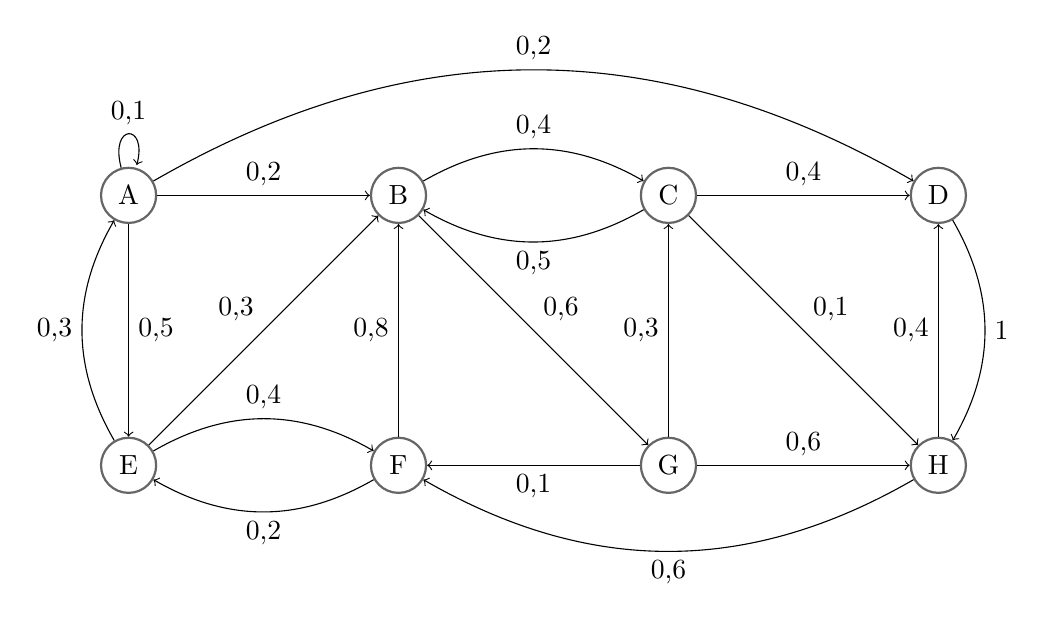
\begin{tikzpicture}[roundnode/.style={circle, draw=black!60, thick, minimum size=7mm}, ->, node distance=2.7cm, auto]
        \node[roundnode]    (nicla)      {A};
        \node[roundnode]    (enka)        [right=of nicla]{B};
        \node[roundnode]    (dvojka)      [right=of enka]{C};
        \node[roundnode]    (trojka)      [right=of dvojka]{D};
        \node[roundnode]    (stirka)      [below=of nicla]{E};
        \node[roundnode]    (petka)      [below=of enka]{F};
        \node[roundnode]    (sestka)      [below=of dvojka]{G};
        \node[roundnode]    (sedmka)      [below=of trojka]{H};


        \path(nicla)edge[loop above]node{0,1}(nicla);
        \path(nicla)edge node{0,2}(enka);
        \path(nicla)edge [bend left]node{0,2}(trojka);
        \path(nicla)edge node{0,5}(stirka);

        \path(enka)edge[bend left]node{0,4}(dvojka);
        \path(enka) edge node{0,6}(sestka);

        \path(dvojka)edge node{0,4}(trojka);
        \path(dvojka)edge[bend left]node{0,5}(enka);
        \path(dvojka)edge node{0,1}(sedmka);

        \path(trojka)edge[bend left]node{1}(sedmka);

        \path(stirka)edge[bend left]node{0,3}(nicla);
        \path(stirka)edge[bend left]node{0,4}(petka);
        \path(stirka)edge node{0,3}(enka);

        \path(petka)edge[bend left]node{0,2}(stirka);
        \path(petka)edge node{0,8}(enka);

        \path(sestka)edge node{0,3}(dvojka);
        \path(sestka)edge node{0,6}(sedmka);
        \path(sestka)edge node{0,1}(petka);

        \path(sedmka)edgenode{0,4}(trojka);
        \path(sedmka)edge[bend left]node{0,6}(petka);



    \end{tikzpicture}
\end{center}

Definiramo slučajno spremenljivko $T$ s porazdelitvijo
$$
T \sim min\{n \ge 1, X_n = D\}
,
$$
ki nam pove kdaj smo prvič prišli na postajo $D$ in je čas ustavljanja. Če bi $T$ definirali, da bi zavzel vrenost natanko tri
postaje pred prvim prihodom na postajo $D$, nebi ustrezal definiciji časa ustavljanja, saj bi upošteval stanja $X_0, X_1, ... X_n, X_{n+1}, X_{n+2}, X_{n+3}.$
Če bi pa $T$ definirali, da zavzame vrednost pet postaj po prvem prihodu na postajo $D$, bi to vselej bil čas ustavljanja, saj bi upoštevali samo 
stanja $X_0, X_1, ..., X_{n-5}.$

\begin{definicija}
    Slučajno spremenljivko $T_s = min\{n \ge 1, X_n = s\}$, kjer je $s \in S$ začetno stanje ($X_0 = s$), imenujemo \textbf{čas prvega povratka}, 
    torej čas, ko se markovska veriga prvič ponovno vrne v stanje $s$. 
\end{definicija}

\begin{definicija}
    Slučajno spremenljivko $T^k_s = min\{ n > T^{k-1}_s, X_n = s\}$, kjer je $s \in S$ začetno stanje ($X_0 = s$), imenujemo \textbf{čas} $k$\textbf{-tega povratka}, 
    torej čas, ko se markovska veriga $k$-tič ponovno vrne v stanje $s$.
\end{definicija}

Pokažimo, da je $T^k_s$ res čas ustavljanja z indukcijo po $k$.

\begin{proof}
$k = 1:$
\newline
V primeru ko je $k = 1$, je $T^1_s$ kar čas prvega povratka v stanje $s$ in ga lahko zapišemo kot $T_s = min\{n \ge 1, X_n = s\}$. 
Očitno je $T_s$ odvisen le od stanj $X_0, X_1, ... X_n$ in je torej čas ustavljanja. 

$k \rightarrow k + 1:$
\newline
Po krepki lastnosti Markova lahko $T^{k + 1}_s = min\{ n > T^{k}_s, X_n = s\}$ zapišemo kot $T^k_s = min\{ n > T^{k - 1}_s, X_n = s\}$ + $T_s = min\{n \ge 1, X_n = s\}$.

\end{proof}




\newpage
\section{Klasifikacija stanj}

Ko opazujemo markovsko verigo $X_0, X_1, ...$, se vprašamo, kaj se lahko zgodi z določenim stanjem $s \in S$, ko mini veliko časa?
Intuitivno bi bilo mišljenje, da se bomo nekoč vrnili nazaj v stanje $s$. Mogoče pa se nikoli ne bomo vrnili.
Izkaže se, da se zgodi natanko ena izmed teh dveh opcij.

\begin{definicija}
    Stanje $s \in S$ je \textbf{minljivo}, če velja, da ko začnemo markovsko verigo v tem stanju, se s pozitivno verjetnostjo zgodi, da se veriga nikoli več ne vrne vanj. 
    Torej $P_s(T_s = \infty) > 0$ oziroma $P_s(T_s < \infty) < 1$.
\end{definicija}

\begin{definicija}
    Stanje $s \in S$  je \textbf{povrnljivo}, če velja, da ko začnemo markovsko verigo v tem stanju, se bo veriga skoraj gotovo vrnila vanj. \newline
     Torej $P_s(T_s = \infty) = 0$ oziroma $P_s(T_s < \infty) = 1$.
\end{definicija}


\begin{zgled}
    Vrnimo se na primer kockarjevega proprada za $N=4$ in si poglejmo katera izmed stanj so minljiva ter katera so povrnljiva.
\end{zgled}

    \begin{center}
        \begin{tabular}{ >{\bfseries}c c c c c c }
          & $\mathbf{0}$ & $\mathbf{1}$ & $\mathbf{2}$ & $\mathbf{3}$ & $\mathbf{4}$\\ 
         0 & 1 & 0 & 0 & 0 & 0 \\  
         1 & ,6 & 0 & ,4 & 0 & 0 \\
         2 & 0 & ,6 & 0 & ,4 & 0 \\
         3 & 0 & 0 & ,6 & 0 & ,4 \\
         4 & 0 & 0 & 0 & 0 & 1                    
        \end{tabular}
    \end{center}

Za lažjo predstavo lahko markovko vrigo prikažemo z usmerjenim grafom.

    \begin{center}
        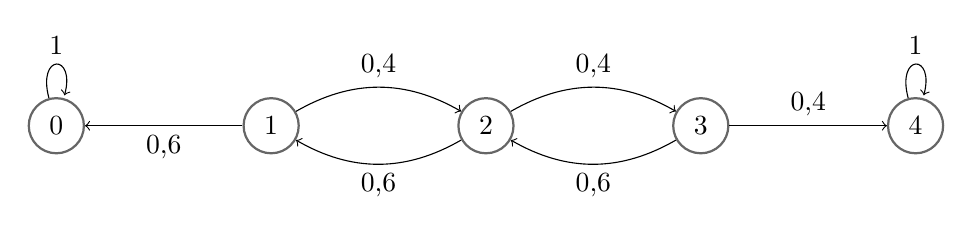
\begin{tikzpicture}[roundnode/.style={circle, draw=black!60, thick, minimum size=7mm}, ->, node distance=2cm, auto]
            \node[roundnode]    (nicla)      {0};
            \node[roundnode]    (enka)        [right=of nicla]{1};
            \node[roundnode]    (dvojka)      [right=of enka]{2};
            \node[roundnode]    (trojka)      [right=of dvojka]{3};
            \node[roundnode]    (stirka)      [right=of trojka]{4};
    
            \path(nicla)edge[loop above]node{1}(nicla);
            \path(stirka)edge[loop above]node{1}(stirka);
            \path(enka)edge[bend left]node{0,4}(dvojka);
            \path(dvojka)edge[bend left]node{0,4}(trojka);
            \path(enka) edge node{0,6} (nicla);
            \path(trojka) edge node{0,4}(stirka);
            \path(trojka) edge[bend left] node{0,6} (dvojka);
            \path(dvojka) edge[bend left] node{0,6} (enka);
        \end{tikzpicture}
    \end{center}

Ko začnemo markovsko verigo v stanju 1, vidimo, da lahko pridemo
z verjetnostjo $0{,}6$ v stanje 0. 0 imenujemo absorbirajoče stanje, ker ko enkrat veriga pride vanj, tam ostane za vedno.
To pa pomeni, da je stanje 1 minljivo, saj obstaja pozitivna verjetnost, da se nikoli ne bomo vrnili vanj. 
S podobnim razmislekom vidimo, da sta tudi 2 in 3 minljivi stanji. Če pogledamo stanje 0, vidimo, da če začnemo
markovsko verigo v njem, ker je absorbirajoče, nikoli ne bomo prešli v katerokoli drugo stanje. To pa pomeni da je stanje 0
povrnljivo. Enak ramislek nam pove, da je tudi 4 povrnljivo stanje.


\begin{zgled}
    (Prehod med generacijami)Naj bo $X_n$ družbeni položaj družine v $n-ti$ generaciji, ki je lahko 1 = $nizek$, 2 = $srednji$ in 3 = $visok$. 
    Naj bo markovska veriga $X_0, X_1, ...$ predstavljena z naslednjo tabelo oz. matriko.
\end{zgled}

\begin{center}
    \begin{tabular}{ >{\bfseries}c c c c }
       & $\mathbf{1}$ & $\mathbf{2}$ & $\mathbf{3}$ \\   
     1 & {,}7 & {,}2 & {,}1 \\
     2 & {,}3 & {,}5 & {,}2 \\
     3 & {,}2 & {,}4 & {,}4 
    \end{tabular}
\end{center}

V tem primeru formalno dokažimo, da so vsa stanja povrnljiva.

\begin{proof}

Ker želimo pokazati, da se bomo nekoč v poljubno stanje $s \in S$, $S=\{1, 2, 3\}$ gotovo vrnili, lahko to pišemo kot
verjetnsot, da bo čas prvega povratka neskončen enaka 0, torej
 $$P_s(T_s = \infty) = 0.$$

Množico dogodkov, ki ustrezajo iskani verjentosti zapišemo kot
$$\{T_s = \infty\} = \{ X_1 \neq s, X_2 \neq s, ...\}.$$



Definiramo množice $$A_n := \{X_1 \neq s, X_2 \neq s, ..., X_n \neq s\}$$ za katere velja 
$$A_1 \supseteq A_2 \supseteq ... \ \ \ \ \  in \ \ \ \ \  \bigcap_{n = 1}^{\infty}A_n = \{T_s = \infty\}.$$



Za vsak $t \in S$ velja ocena
\begin{align*}
    \lefteqn{P_s(A_{n-1} \cap \{X_n = t, X_{n+1}=s\})=} \qquad
    \\& = P_s(A_{n-1} \cap \{X_n = t\}) \cdot p(t,s) \ge
    \\& \ge 0{,}1 \cdot P_s(A_{n-1} \cap \{X_n = t\}) 
\end{align*}


    Ker neenakost velja za vsak $t$, če seštejemo verjetnosti po vseh $t \in S\setminus\{s\}$, se ta ohrani in velja 
\begin{align*}
    \lefteqn{P_s(A_{n-1} \cap \{X_n \neq s, X_{n+1} = s \}) \ge} \qquad
    \\& \ge 0{,}1 \cdot P_s(A_{n-1} \cap \{X_n \neq s\}). 
\end{align*}
Torej velja
 $$P_s(A_n \cap \{ X_{n+1} = s\}) \ge 0{,}1 \cdot P_s(A_n).$$ 



Neenakost uporabimo pri naslednji oceni 
    $$ P_s(A_{n+1}) = P_s(A_n) - P_s(A_n \cap \{X_{n+1} = s\})\le 0{,}9 \cdot P_s(A_n). $$
Z enakim razmislekom lahko ocenimo tudi $P_s(A_n) \le 0{,}9 \cdot P_s(A_{n-1})$ in tako vse do $P_s(A_1)$. Velja
    $$P_s(A_n) \le 0{,}9^n$$
in ko $n \rightarrow \infty$ gre $P_s(A_n) \rightarrow 0$, kar pa pomeni, da je $P_s(T_s = \infty) = 0.$

\end{proof}





\newpage
\section{Lastnosti minljivih in povrnljivih stanj}

Glede na lastnosti markovskih verig se zdi smiselno, da obstaja nekakšna povezava med časom prve in časom 
$k$-te povrnitve v stanje $s \in S$, saj ko se enkrat vrnemo vanj v času $T_s$, po krepki lastnosti Markova velja da stanja $X_0, X_1, ..., X_{T_s-1}$ nimajo 
vpliva na prehod iz $X_{T_s}=s$ v $X_{T_s+1}$.

\begin{trditev}
    Naj bo $X_0, X_1, ...$ markovska veriga z neko prehodno matriko $p(i,j)$ in naj bo $s \in S$ začetno stanje.
    Naj bo $T_s$ čas prvega povratka v stanje $s$ in $T^k_s$ čas $k$-tega povratka. Potem velja
    $$ P_s(T^k_s < \infty) = (P_s(T_s < \infty))^k $$
\end{trditev}

\begin{proof}
    Dokaz temelji na krepki lastnosti Markova.
    $$\{T^k_s< \infty\} \subseteq \{ T_s < \infty\}$$
    $$P_s(T^k_s < \infty) = P_s(T_s < \infty) \cdot P_s(T^k_s < \infty \mid T_s < \infty)$$
    pogojno na $\{T_s < \infty \} = \{X_{T_s} = s\}$ je 
    $X_{T_s}, X_{T_{s+1}}, ...$ spet markovska veriga s prehodno matriko $p(i,j)$, ki se začne v $s$. \newline
    Zato je $$P_s(T^k_s < \infty \mid T_s < \infty) = P_s(T^{k-1}_s < \infty)$$ 
    $$P_s(T^k_s < \infty) = P_s(T_s < \infty) \cdot P_s(T^{k-1}_s < \infty)$$
    Z indukcijo po $k$ se dokončno dokaže, da $ P_s(T^k_s < \infty) = (P_s(T_s < \infty))^k $.
\end{proof}

Sedaj lahko pokažemo ključni lastnosti minljivih in povrnljivih stanj v markovskih verigah.

Če je stanje minljivo, potem velja, da se markovska veriga vrne vanj le končno mnogokrat.
$$P_s(\bigcup_{k=1}^{\infty}\{T^k_s = \infty\}) = 1 \iff P_s(\bigcap_{k = 1}^{\infty}\{T_s^k < \infty\}) = 0$$ 

Če je stanje povrnljivo, potem velja, da se markovska veriga vrne vanj neskončno mnogokrat.
$$P_s(\bigcap_{k=1}^{\infty}\{T^k_s < \infty\}) = 1 \iff P_s(\bigcup_{k=1}^{\infty}\{T^k_s = \infty\}) = 0$$

Pokažimo, da za minljiva stanja velja $P_s(\bigcap_{k = 1}^{\infty}\{T_s^k < \infty\}) = 0$.

\begin{proof}

        \begin{align*}
            \lefteqn{P_s(\bigcap_{k = 1}^{\infty}\{T_s^k < \infty\}) =} \qquad
            \\& = \lim_{k \to \infty}P_s(\{T_s^k < \infty\}) = 
            \\& = \lim_{k \to \infty}P_s(\{T_s < \infty\})^k
        \end{align*}

Ker je stanje $s$ minljivo velja $P_s(\{T_s<\infty\}) < 1$. Torej ko $k \rightarrow \infty$ gre
$P_s(\{T_s < \infty\})^k \rightarrow 0.$ Podoben argument velja za ostale tri enakosti.
\end{proof}



\nocite{RickDurrett}
\nocite{MatjazOmladic_1}
\nocite{MatjazOmladic_2}


\pagebreak



\bibliography{Naloga-Anej_Rozman}
\addcontentsline{toc}{section}{Literatura}
\bibliographystyle{plain}

\end{document}